\section{Artefact}\label{sec:artefact}
This section describes the NetLogo model created, `FoodDelivery'.

The world being modeled is what is known as the last mile in the food delivery industry.
This term is used for the last step in the delivery of online-ordered goods.

Companies in the food delivery industry offer a service to three parties:
\begin{itemize}
    \item restaurants sell their food in a portal made by the delivery company.
    \item consumers buy food from a restaurant using the same portal.
    \item a mobile app from the delivery company steers deliverers.
\end{itemize}

The steps in the food ordering and delivery process are:
\begin{itemize}
    \item When a customer orders a meal, a message is sent to the restaurant.
    \item The restaurant starts preparing the meal; this may take some time (say, on average, 10 minutes).
    \item When it starts preparing, a deliverer is needed.
    \item A deliverer can claim the delivery (or is assigned) and starts cycling towards the restaurant.
    \item When the deliverer arrives at the restaurant, it may have to wait until the meal is ready.
    \item When the meal is ready, the deliverer takes it and starts driving towards the customer.
    \item It is possible no deliverer is available, or it takes too long to get to the restaurant,
then the meal will be thrown away.
    \item If the meal gets delivered, the customer is happy
    \item If the meal is not delivered, the customer is unhappy.
    \item If a customer is unhappy, it will eventually stop ordering meals.
\end{itemize}

This all takes place in a city with restaurants and customers.
The deliverers have to cycle to the restaurant and then to the customer.
The best route will be provided by the app the deliverers use.

The money for the delivery company is earned by charging the restaurants per delivery.
The company's interest is thus to have as many deliveries as possible; this means they want happy customers and enough deliverers to keep them happy.

The above process is more or less how the process works in the real world.

\subsection{Conceptional model}\label{subsec:conceptional-model}
The FoodDelivery model has the same types of agents:
-deliverers \\
-restaurants \\
-customers \\

The delivery company itself is not modeled explicitly; they are what is called the observer.

\paragraph{Customers} will order food from a restaurant.
Orders are not equally distributed per day, peak hours are breakfast, lunch, and dinner.
They will, on average, order once a week.
The restaurant is selected at random.
The probability distribution shown in figure~\ref{fig:food_ordering_distribution} is used in the model.
If a meal is not delivered, the customer is unsatisfied, and their satisfaction level is subtracted 1 point.
Customers stop ordering food if they have a satisfaction level below -1.

\begin{figure}
    \centering
    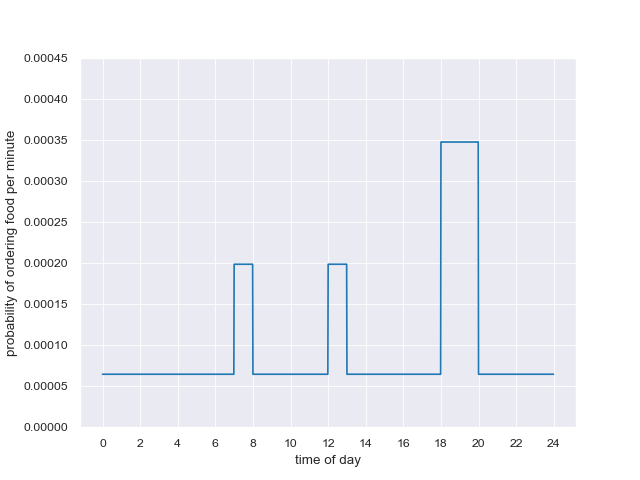
\includegraphics[width=8.5cm]{sections/pics/food_ordering_distribution}
    \caption{food ordering probabilities for one day}
    \label{fig:food_ordering_distribution}
\end{figure}

\paragraph{Restaurants} accept any order and are always open.
When an order arrives, the preparation starts.
This preparation time is Gaussian distributed, and the mean and standard deviation can be set.
Upon order arrival, the meal can be assigned to a deliverer.
When the meal is ready, it can be picked up for a waiting time that can be set.
After this waiting time, the meal will be thrown away.

Not in the current model, but what could be interesting are:
-restaurants cannot leave the system if they have not enough orders\\
-the freshness of the meal is not taken into account\\

\paragraph{Deliverers} are the only agents that can move.
Two possible meal distribution strategies can be set:
-distribute meals equally among the deliverers\\
-assign a meal to the closest free deliverer\\

When a meal is assigned to the deliverer, it will take the shortest route
to the restaurant, wait until the meal is ready and move to the customer.
The deliverer will lose its assigned meal if they do not arrive before the waiting time is over.
A deliverer can only receive or deliver a meal when it is neighboring a restaurant or the customer.

As a design choice, deliverers have no shifts; they work all the time.
Using shifts would make the model much more complicated; this could be done in the next version.

\paragraph{The world} consists of a grid of squares; some squares will be blocks of buildings, and others represent the streets.
This grid places restaurants and customers randomly on the building blocks.
The deliverers are initially randomly placed on the streets; they can only move on the street patches.

The delivery company's goal is not profit but to make as many deliveries as possible.

\subsection{Computer model}\label{subsec:computer-model}
The world is, for a large part, built using the code from the Taxi Cab model.
The streets and how the deliveries move are from their model; only the traffic lights were removed.

The design of the grid is show in figure~\ref{fig:grid}.
\begin{center}
\begin{figure*}
    \centering
    \begin{subfigure}[m]{0.6\textwidth}
        \centering
        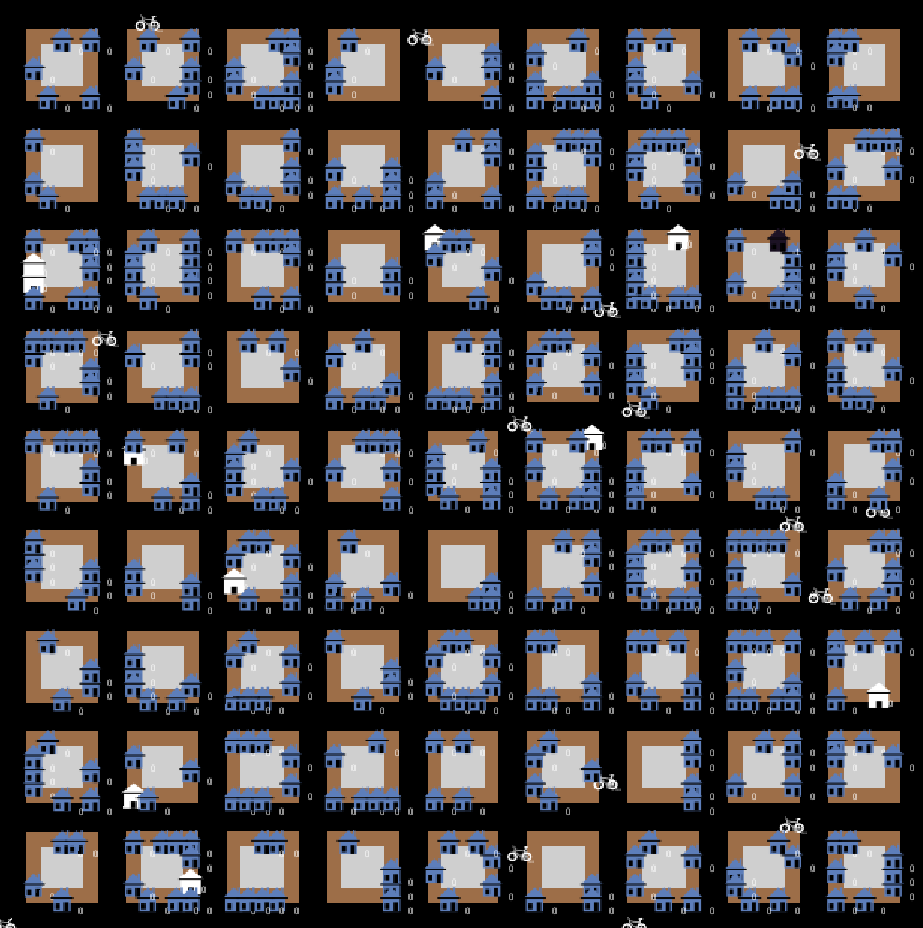
\includegraphics[width=8cm]{sections/pics/grid}
        \caption{FoodDelivery grid}
    \end{subfigure}
    \hfill
    \begin{subfigure}[m]{0.6\textwidth}
        \centering
        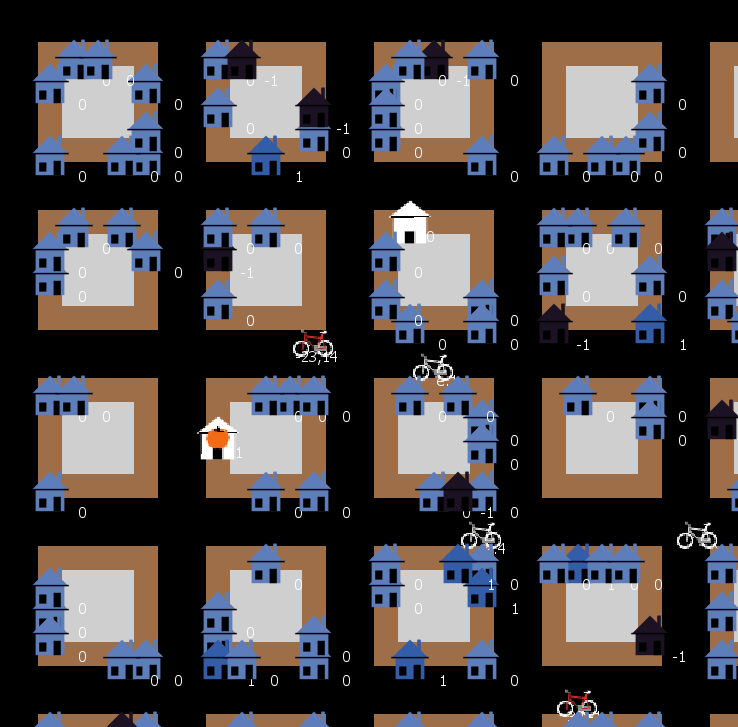
\includegraphics[width=8cm]{sections/pics/grid_closeup}
        \caption{Fooddelivery grid closeup}
    \end{subfigure}
    \caption{FoodDelivery grid}
    \label{fig:grid}
\end{figure*}

\end{center}
The agents design is shown in figure~\ref{fig:agents}.
\begin{center}
\begin{figure}
     \centering
     \begin{subfigure}[m]{0.1\textwidth}
         \centering
         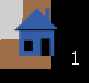
\includegraphics[width=\textwidth]{sections/pics/cust_happy}
         \caption{Customer with happiness score}
     \end{subfigure}
     \hfill
     \begin{subfigure}[m]{0.1\textwidth}
         \centering
         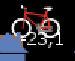
\includegraphics[width=\textwidth]{sections/pics/del_on_its_way}
         \caption{Deliverer on route to loc 23,1}
     \end{subfigure}
     \hfill
     \begin{subfigure}[m]{0.1\textwidth}
         \centering
         
\includegraphics[width=\textwidth]{sections/pics/meal_prep}
         \caption{Restaurant with a meal ordered on top and number of ordered}
     \end{subfigure}
      \hfill
     \begin{subfigure}[m]{0.1\textwidth}
         \centering
         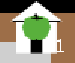
\includegraphics[width=\textwidth]{sections/pics/meal_ready}
         \caption{Restaurant with a meal ready on top and number of ordered}
     \end{subfigure}
        \caption{Agents examples}
        \label{fig:agents}
\end{figure}
\end{center}
In NetLogo, everything works on ticks; all code in the go procedure is executed during one tick.
The programmer must decide what to do and not to do in that tick during programming.
And be sure that each agent does only one thing in a tick.

In one tick, all behavior of one kind of agent is executed in series.
The order of these series is essential.

This system makes it difficult to program future behavior as each agent decides only its behavior one tick at a time.
For example, moving towards a restaurant means moving to an allowed patch that minimizes the distance to that restaurant.

The most important parts of the grid are the squares.
The squares are named patches.

The street patches have four kinds:\\
- right patches where a deliverer can only move right\\
- left patches where a deliverer can only move left\\
- up patches where a deliverer can only move up\\
- down patches where a deliverer can only move down\\

On horizontal roads, the allowed directions are left or right
On vertical roads, the directions are up or down.

Next to road patches, there are intersection patches; on these patches, a driver has more allowed directions.
These are:\\
- up or right\\
- up or left\\
- left or down\\
- right or down\\

At an intersection, a deliverer decides which direction to go.
To get to the other side of the road, the deliverer has to go to an intersection to make a U-turn.

Special patches are the intersections at the edges of the grid; a deliverer can not leave the grid.

Another important detail is that to pick up or deliver a meal, the delivery person must be on a street patch rather than at an intersection.

The program is available inside a git repository available at GitHub~\footnote{\url{https://github.com/evertvankammen/FooddeliveryNetlogo}}
This repository also contains the Python code to automate the model's running with different parameters.h and not on an intersection.
